\chapter{Analyse et Spécification}


\chapteropeningtext{Ce chapitre présente l'analyse fonctionnelle et la spécification des besoins de la solution \textbf{SomaScan}. Après l'étude du contexte général du projet, il s'agit ici de formaliser les acteurs du système, les fonctionnalités attendues, les règles métier, les contraintes non fonctionnelles ainsi que les principaux cas d'utilisation.\par\medskip L'objectif de cette phase est de transformer le besoin métier en exigences claires et exploitables pour la conception. La solution doit permettre à SOMASTEEL de suivre les trajets des camions loués entre l'entreprise et le port, sans recourir à un système GPS. Le suivi repose sur un flux de scans QR, effectué par des opérateurs autorisés, et supervisé par l'agent logistique à travers une application web.}{Analyse des besoins -- Acteurs -- Exigences -- Cas d'utilisation -- Règles métier}

\section{Analyse des besoins}

Le besoin principal concerne la digitalisation du suivi des camions loués utilisés pour transporter la ferraille. Comme ces véhicules n'appartiennent pas à SOMASTEEL, l'entreprise ne peut pas y installer de dispositifs GPS. Le système doit donc proposer une alternative fiable permettant d'enregistrer les étapes importantes du trajet à partir de points de contrôle.

La solution attendue doit centraliser les informations liées aux camions, aux trajets, aux scans et aux utilisateurs. Elle doit également permettre à l'agent logistique de suivre l'activité en temps réel, de consulter les historiques, d'analyser les durées de trajet et d'exporter des rapports exploitables. Pour les opérateurs terrain, l'application doit rester simple : scanner un code QR, recevoir une confirmation ou une erreur, puis consulter l'historique récent des opérations effectuées.

\subsection{Périmètre fonctionnel}

Le périmètre de SomaScan couvre les éléments suivants :

\begin{itemize}
    \item gestion des utilisateurs et de leurs rôles ;
    \item gestion des camions et de leurs codes QR ;
    \item suivi du cycle de vie des trajets ;
    \item exécution des scans au niveau de l'usine et du port ;
    \item consultation des trajets actifs, terminés, annulés et historiques ;
    \item gestion des exceptions comme l'annulation d'un trajet ;
    \item consultation des logs de scan et des historiques opérateurs ;
    \item génération de statistiques, rapports et exports Excel ;
    \item consultation des trajets sous forme de calendrier ;
    \item configuration du flux dynamique des étapes de scan.
\end{itemize}

Le système ne fournit pas une localisation continue du camion. Il enregistre plutôt des événements métier validés par scan : départ de l'usine, arrivée au port, départ du port et retour à l'usine.

\subsection{Données principales manipulées}

Les principales données manipulées par le système sont :

\begin{itemize}
    \item les utilisateurs, avec leur nom, email, mot de passe, rôle et localisation ;
    \item les camions, identifiés par un numéro d'immatriculation unique, un chauffeur, un code QR et un état actif ou inactif ;
    \item les trajets, avec leur camion associé, leur statut, leurs dates de passage, leurs notes et leur état actif ;
    \item les logs de scan, qui enregistrent l'opérateur, le camion, le trajet, l'action, la localisation et la date du scan ;
    \item les étapes du flux de scan, configurables par l'agent logistique.
\end{itemize}

\section{Acteurs du système et besoins fonctionnels}

Le système repose sur trois acteurs principaux. Dans la documentation technique, ces rôles correspondent à \path{ADMIN}, \path{COMPANY_OPERATOR} et \path{PORT_OPERATOR}. Dans le rapport, ils sont nommés respectivement \textbf{agent logistique}, \textbf{opérateur usine} et \textbf{opérateur port}.

\subsection{Acteurs du système}

\begin{longtable}{|p{3.4cm}|p{3.5cm}|p{7cm}|}
\hline
\textbf{Acteur} & \textbf{Localisation} & \textbf{Rôle principal} \\
\hline
\endhead

Agent logistique & Back-office / application web & Supervise l'ensemble du système, gère les utilisateurs, les camions, les trajets, les logs, les rapports et la configuration du flux de scan. \\
\hline

Opérateur usine & Usine / dépôt de l'entreprise & Scanne les camions au départ de l'entreprise pour démarrer un trajet et au retour du camion pour clôturer le trajet. \\
\hline

Opérateur port & Point de contrôle au port & Scanne les camions lors de leur arrivée au port et lors de leur départ du port. \\
\hline

\caption{Acteurs principaux du système SomaScan}
\label{tab:acteurs-somascan}
\end{longtable}

La figure~\ref{fig:acteurs-systeme} représentera les acteurs principaux et leur interaction générale avec SomaScan.

\begin{figure}[H]
    \centering
    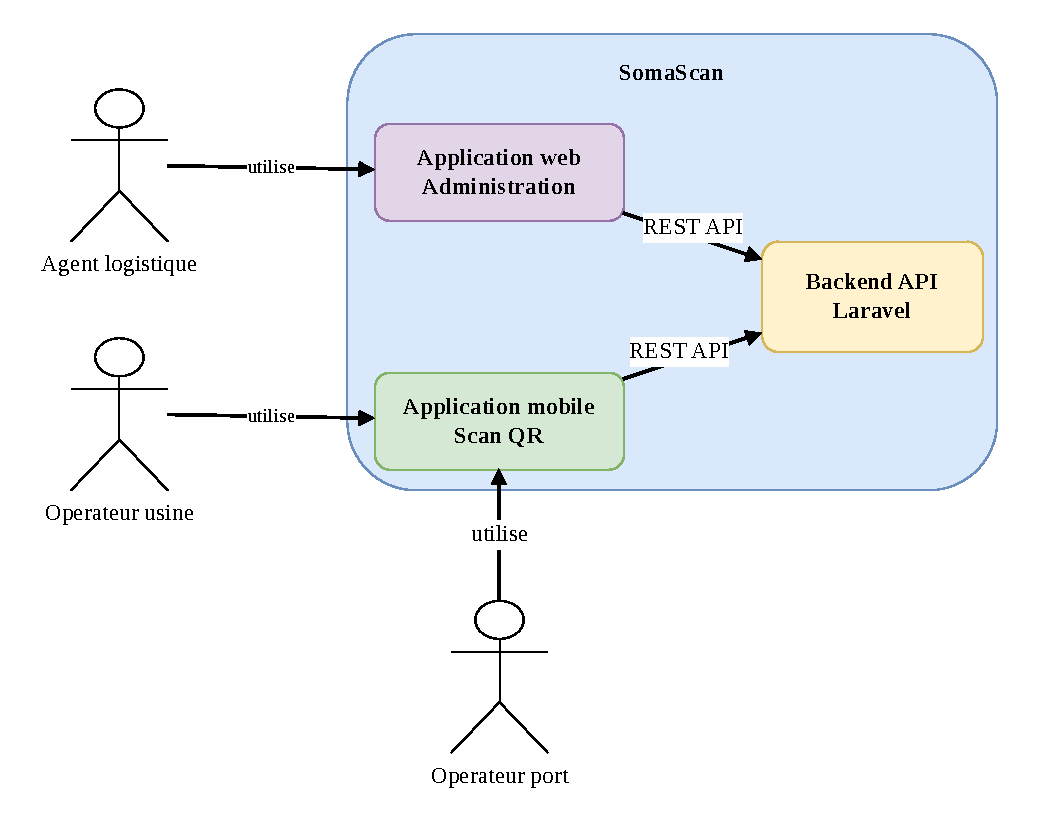
\includegraphics[width=\textwidth]
    {figures/diagrams/diagramme-des-acteurs.pdf}

    \caption{Diagramme des acteurs du système SomaScan}

    \label{fig:acteurs-systeme}
\end{figure}

\subsection{Besoins fonctionnels de l'agent logistique}

L'agent logistique possède le rôle le plus complet du système. Ses besoins fonctionnels sont les suivants :

\begin{itemize}
    \item gérer les utilisateurs : création, modification, recherche, consultation des statistiques, activité et réinitialisation des mots de passe ;
    \item gérer les camions : ajout, modification, activation, désactivation, suppression, recherche, statistiques et consultation des trajets d'un camion ;
    \item générer, télécharger ou régénérer les codes QR des camions ;
    \item consulter le tableau de bord global : nombre de camions, trajets, utilisateurs, trajets actifs et trajets du jour ;
    \item suivre les trajets actifs, terminés, annulés et historiques ;
    \item rechercher et filtrer les trajets selon plusieurs critères ;
    \item consulter le détail d'un trajet et sa chronologie de scans ;
    \item annuler un trajet actif avec ajout d'une note explicative ;
    \item ajouter ou mettre à jour des notes sur un trajet ;
    \item supprimer un trajet lorsque cela est nécessaire pour le nettoyage des données ;
    \item consulter les logs de scan globaux avec filtres et statistiques ;
    \item générer des rapports analytiques et des exports Excel ;
    \item consulter les trajets sous forme de calendrier avec détail par journée ;
    \item configurer l'ordre des étapes du flux de scan.
\end{itemize}

\subsection{Besoins fonctionnels de l'opérateur usine}

L'opérateur usine utilise l'application mobile sur le site de l'entreprise. Ses besoins fonctionnels sont :

\begin{itemize}
    \item s'authentifier sur l'application mobile ;
    \item scanner le QR code d'un camion pour démarrer un trajet ;
    \item scanner le QR code d'un camion à son retour à l'usine afin de clôturer le trajet ;
    \item consulter les informations de base du camion après résolution du QR code ;
    \item consulter son historique récent de scans ;
    \item recevoir un message clair en cas de succès ou d'erreur.
\end{itemize}

\subsection{Besoins fonctionnels de l'opérateur port}

L'opérateur port utilise également l'application mobile, mais ses actions sont limitées au point de contrôle du port :

\begin{itemize}
    \item s'authentifier sur l'application mobile ;
    \item scanner le QR code d'un camion pour enregistrer son arrivée au port ;
    \item scanner le QR code d'un camion pour enregistrer son départ du port ;
    \item consulter les informations de base du camion après résolution du QR code ;
    \item consulter son historique récent de scans ;
    \item recevoir un message clair en cas de succès ou d'erreur.
\end{itemize}

\subsection{Règles métier principales}

Les règles métier assurent la cohérence du suivi des trajets :

\begin{itemize}
    \item chaque camion possède un numéro d'immatriculation unique ;
    \item le code QR est généré selon le format \texttt{SOMASTEEL-TRUCK-}\path{IMMATRICULATION_NORMALISEE} ;
    \item le numéro d'immatriculation est normalisé en majuscules, avec remplacement des caractères non alphanumériques par des tirets ;
    \item un camion inactif ne peut pas être scanné ;
    \item un camion ne peut pas avoir deux trajets actifs en même temps ;
    \item le flux par défaut est \path{STARTED} vers \path{ARRIVED_PORT}, puis \path{LEFT_PORT}, puis \path{COMPLETED} ;
    \item la dernière étape du flux doit toujours être \path{COMPLETED} ;
    \item les étapes du flux doivent être uniques et correspondre à des statuts valides ;
    \item seul l'opérateur usine peut démarrer et clôturer un trajet ;
    \item seul l'opérateur port peut enregistrer l'arrivée et le départ du port ;
    \item un scan effectué par le mauvais rôle ou dans le mauvais ordre est rejeté avec un message d'erreur ;
    \item chaque scan valide doit créer un log de scan ;
    \item les opérations de scan se font en ligne afin de valider immédiatement le statut du trajet ;
    \item l'annulation d'un trajet libère le camion pour un futur trajet ;
    \item les trajets annulés ne sont pas considérés comme retardés dans l'analyse.
\end{itemize}

\section{Besoins non fonctionnels}

En plus des fonctionnalités métier, SomaScan doit satisfaire plusieurs exigences de qualité.

\begin{longtable}{|p{4cm}|p{10cm}|}
\hline
\textbf{Besoin} & \textbf{Description} \\
\hline
\endhead

Sécurité & L'accès au système doit être protégé par authentification. Les opérations sont limitées selon le rôle de l'utilisateur. Les mots de passe sont stockés de manière sécurisée et les accès API reposent sur des jetons d'authentification. \\
\hline

Traçabilité & Toutes les opérations de scan doivent être enregistrées avec l'utilisateur, le camion, le trajet, l'action, la localisation et la date du scan. \\
\hline

Cohérence & Le système doit empêcher les transitions invalides, les scans hors séquence, les scans sur camions inactifs et les doublons de trajets actifs. \\
\hline

Disponibilité en ligne & Les scans nécessitent une connexion afin de vérifier immédiatement le camion, le trajet actif et l'action autorisée. \\
\hline

Performance & La résolution du QR code, la validation du scan et la mise à jour du trajet doivent être rapides pour ne pas ralentir les opérateurs sur le terrain. \\
\hline

Fiabilité concurrente & Lors d'un scan, le trajet actif doit être verrouillé côté backend afin d'éviter les incohérences en cas de requêtes simultanées. \\
\hline

Ergonomie & L'application mobile doit être simple, lisible et adaptée à une utilisation opérationnelle rapide. L'application web doit faciliter la recherche, le filtrage et le suivi. \\
\hline

Maintenabilité & Le flux de scan doit rester configurable afin d'adapter l'application à une évolution du processus métier. \\
\hline

Exploitabilité & Les données doivent pouvoir être filtrées, recherchées, exportées et utilisées pour produire des indicateurs de suivi. \\
\hline

\caption{Besoins non fonctionnels de SomaScan}
\label{tab:besoins-non-fonctionnels}
\end{longtable}

\section{Diagramme de cas d'utilisation et descriptions}

La figure~\ref{fig:use-case-global} représentera le diagramme de cas d'utilisation global. Elle regroupera les trois acteurs principaux et les fonctionnalités majeures du système.

\begin{figure}[H]
    \centering
    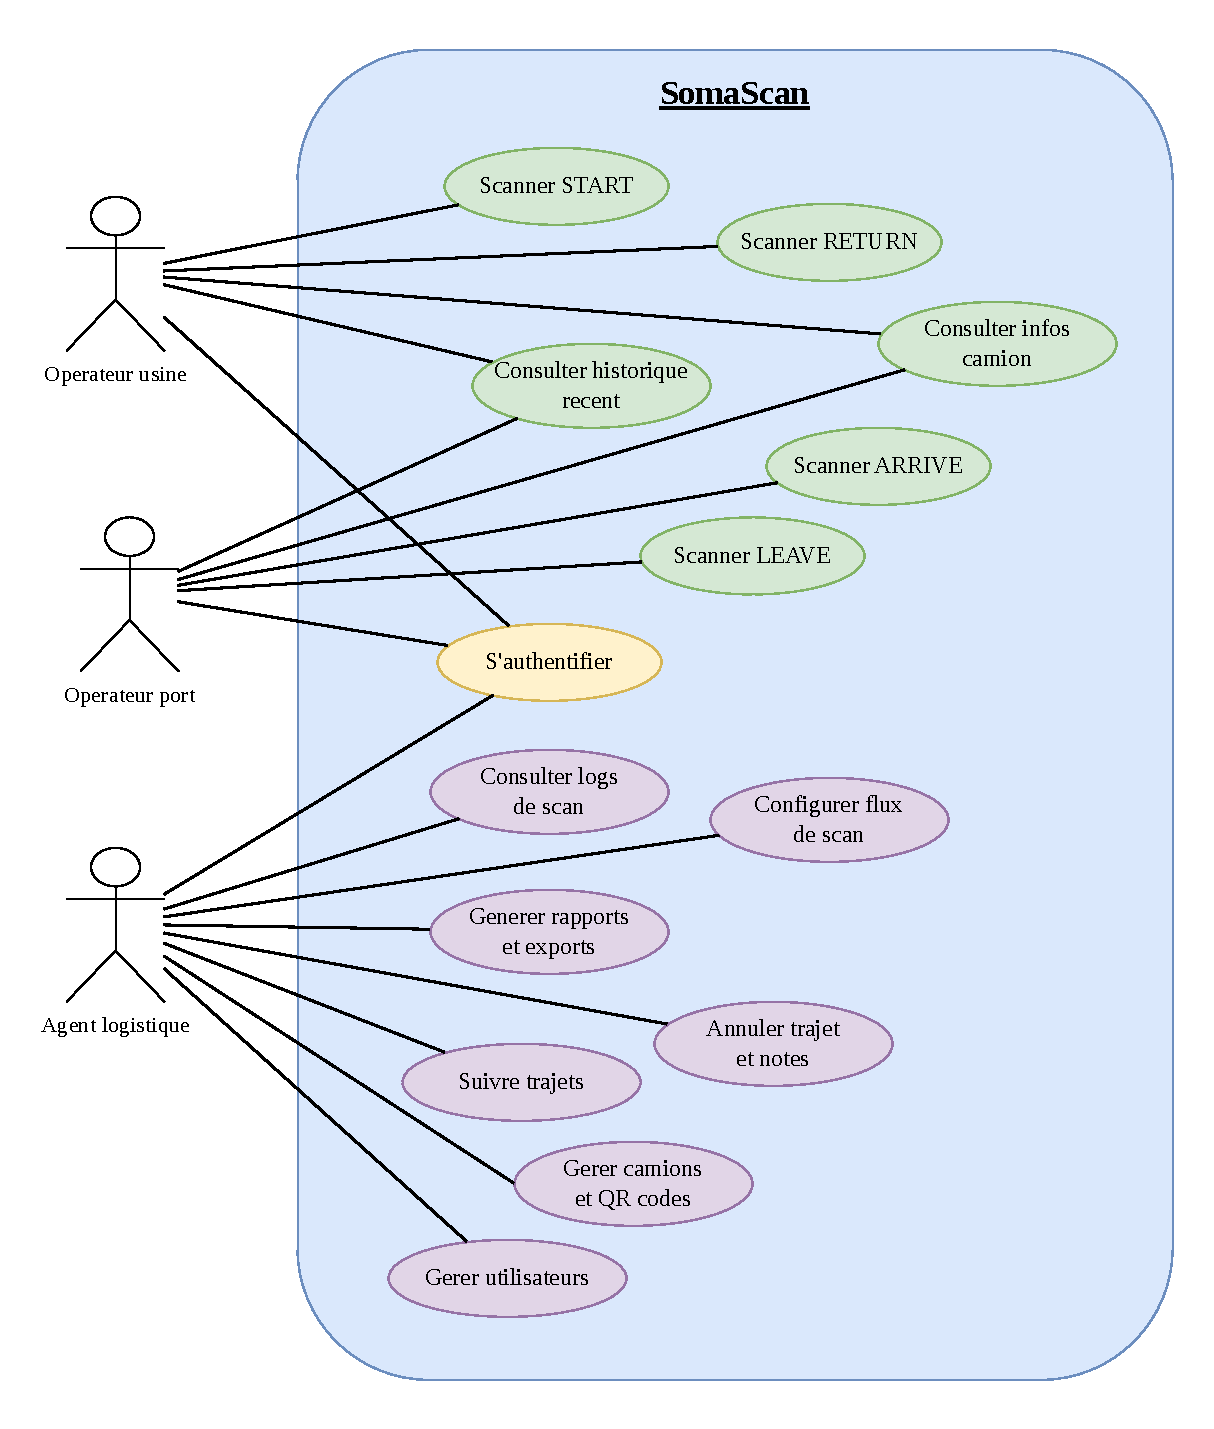
\includegraphics[width=\textwidth]
    {figures/diagrams/diagramme-de-cas-utilisation.pdf}

    \caption{Diagramme de cas d'utilisation de SomaScan}

    \label{fig:use-case-global}
\end{figure}

Les cas d'utilisation détaillés sont présentés sous forme de tableaux afin de décrire les scénarios, les préconditions, les exceptions et les résultats attendus.

\subsection{UC01 : Authentification et session}

\begin{longtable}{|p{4cm}|p{10cm}|}
\hline
\textbf{Élément} & \textbf{Description} \\
\hline
\endhead

Acteurs & Agent logistique, opérateur usine, opérateur port. \\
\hline
Objectif & Permettre à un utilisateur d'accéder à l'application selon son rôle. \\
\hline
Scénario nominal & L'utilisateur saisit son email et son mot de passe. Le système vérifie les identifiants, retourne un jeton d'accès, le profil utilisateur et les informations de session. \\
\hline
Exceptions & Si les identifiants sont incorrects ou si le compte est invalide, l'accès est refusé. \\
\hline
Résultat & L'utilisateur authentifié accède aux fonctionnalités autorisées. \\
\hline
\caption{UC01 : Authentification et session}
\label{tab:uc-authentification}
\end{longtable}

\subsection{UC02 : Gestion des utilisateurs}

\begin{longtable}{|p{4cm}|p{10cm}|}
\hline
\textbf{Élément} & \textbf{Description} \\
\hline
\endhead

Acteur principal & Agent logistique. \\
\hline
Objectif & Administrer les comptes des utilisateurs du système. \\
\hline
Scénario nominal & L'agent logistique crée, modifie, recherche ou consulte les utilisateurs. Il peut filtrer par rôle ou localisation, consulter les statistiques, voir l'activité d'un utilisateur et réinitialiser son mot de passe. \\
\hline
Exceptions & Un email déjà utilisé ou un mot de passe invalide entraîne le rejet de l'opération. \\
\hline
Résultat & Les comptes utilisateurs sont correctement maintenus et associés aux bons rôles. \\
\hline
\caption{UC02 : Gestion des utilisateurs}
\label{tab:uc-gestion-utilisateurs}
\end{longtable}

\subsection{UC03 : Gestion des camions et des QR codes}

\begin{longtable}{|p{4cm}|p{10cm}|}
\hline
\textbf{Élément} & \textbf{Description} \\
\hline
\endhead

Acteur principal & Agent logistique. \\
\hline
Objectif & Enregistrer les camions et gérer leurs codes QR. \\
\hline
Scénario nominal & L'agent logistique saisit le numéro d'immatriculation et le nom du chauffeur. Le système vérifie l'unicité, enregistre le camion et génère un code QR déterministe. L'agent peut mettre à jour le camion, l'activer, le désactiver, le supprimer, le rechercher ou régénérer son QR code. \\
\hline
Exceptions & Si le camion est inactif, les scans sont refusés. Si le numéro d'immatriculation existe déjà, l'enregistrement est rejeté. \\
\hline
Résultat & Le camion est disponible dans le système et identifiable par son QR code. \\
\hline
\caption{UC03 : Gestion des camions et des QR codes}
\label{tab:uc-gestion-camions}
\end{longtable}

\subsection{UC04 : Cycle de vie d'un trajet}

Le cycle de vie d'un trajet constitue le coeur fonctionnel de SomaScan. Il agit comme une machine à états configurable. La figure~\ref{fig:cycle-vie-expedition} représentera ce cycle.

\begin{figure}[H]
    \centering
    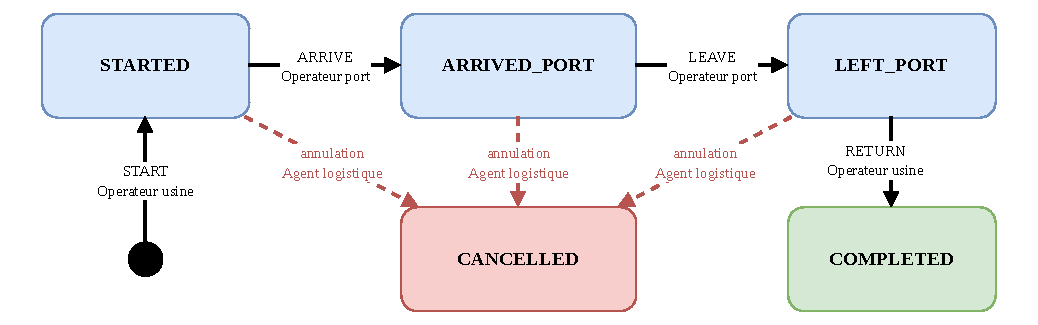
\includegraphics[width=\textwidth]
    {figures/diagrams/diagramme-etats-transition-trajet.pdf}

    \caption{diagramme d'états-transitions - Cycle de vie des statuts d'un trajet}

    \label{fig:cycle-vie-expedition}
\end{figure}

\begin{longtable}{|p{3.2cm}|p{5.8cm}|p{5cm}|}
\hline
\textbf{Étape} & \textbf{Action} & \textbf{Résultat} \\
\hline
\endhead

Départ usine & L'opérateur usine scanne le QR code du camion. & Création d'un trajet avec le statut \path{STARTED} et log \path{START}. \\
\hline

Arrivée port & L'opérateur port scanne le QR code à l'arrivée du camion au port. & Passage au statut \path{ARRIVED_PORT} et log \path{ARRIVE}. \\
\hline

Départ port & L'opérateur port scanne le QR code lorsque le camion quitte le port. & Passage au statut \path{LEFT_PORT} et log \path{LEAVE}. \\
\hline

Retour usine & L'opérateur usine scanne le QR code au retour du camion. & Passage au statut \path{COMPLETED}, clôture du trajet et log \path{RETURN}. \\
\hline

\caption{Étapes principales du cycle de vie d'un trajet}
\label{tab:cycle-vie-trajet}
\end{longtable}

\subsection{UC05 : Annulation, suppression et notes de trajet}

\begin{longtable}{|p{4cm}|p{10cm}|}
\hline
\textbf{Élément} & \textbf{Description} \\
\hline
\endhead

Acteur principal & Agent logistique. \\
\hline
Objectif & Gérer les exceptions liées aux trajets. \\
\hline
Scénario nominal & En cas de panne ou d'abandon, l'agent logistique annule le trajet actif. Le statut devient \path{CANCELLED}, le trajet n'est plus actif et une note explicative peut être ajoutée. L'agent peut également mettre à jour les notes d'un trajet actif ou terminé. \\
\hline
Action destructive & La suppression définitive d'un trajet est possible pour les besoins de nettoyage des données. \\
\hline
Résultat & L'historique reste exploitable et le camion peut être réutilisé pour un futur trajet après annulation. \\
\hline
\caption{UC05 : Gestion des exceptions de trajet}
\label{tab:uc-exceptions-trajet}
\end{longtable}

\subsection{UC06 : Suivi, recherche et calendrier des trajets}

\begin{longtable}{|p{4cm}|p{10cm}|}
\hline
\textbf{Élément} & \textbf{Description} \\
\hline
\endhead

Acteur principal & Agent logistique. \\
\hline
Objectif & Suivre l'activité logistique à travers les trajets. \\
\hline
Scénario nominal & L'agent logistique consulte les trajets avec pagination et filtres, visualise les trajets actifs, terminés ou annulés, ouvre le détail d'un trajet, consulte la chronologie des scans et effectue des recherches. \\
\hline
Vue calendrier & Le système permet une synthèse journalière des trajets avec une limite de journée configurable et une gestion du fuseau horaire. \\
\hline
Résultat & L'agent dispose d'une vision claire des opérations par trajet, par camion et par période. \\
\hline
\caption{UC06 : Suivi et consultation des trajets}
\label{tab:uc-suivi-trajets}
\end{longtable}

\subsection{UC07 : Audit des scans}

\begin{longtable}{|p{4cm}|p{10cm}|}
\hline
\textbf{Élément} & \textbf{Description} \\
\hline
\endhead

Acteurs & Agent logistique, opérateur usine, opérateur port. \\
\hline
Objectif & Consulter les historiques de scans. \\
\hline
Scénario nominal & L'agent logistique consulte tous les logs de scan avec filtres par opérateur, camion, trajet, rôle, localisation, action, date ou recherche libre. Les opérateurs terrain consultent uniquement leur historique récent de scans. \\
\hline
Résultat & Les opérations sont traçables et exploitables pour l'audit et le suivi. \\
\hline
\caption{UC07 : Audit et historique des scans}
\label{tab:uc-audit-scans}
\end{longtable}

\subsection{UC08 : Reporting et analytics}

\begin{longtable}{|p{4cm}|p{10cm}|}
\hline
\textbf{Élément} & \textbf{Description} \\
\hline
\endhead

Acteur principal & Agent logistique. \\
\hline
Objectif & Générer des indicateurs et des exports exploitables. \\
\hline
Scénario nominal & L'agent logistique sélectionne une période ou un camion. Le système calcule les statistiques de trajets, les durées moyennes et les durées par segment : entreprise-port, durée au port, port-entreprise et durée totale. \\
\hline
Export & Le système génère un fichier Excel avec des en-têtes en français et les informations principales des trajets. \\
\hline
Résultat & Les données historiques peuvent être analysées et partagées avec la direction. \\
\hline
\caption{UC08 : Reporting et analytics}
\label{tab:uc-reporting}
\end{longtable}

\subsection{UC09 : Consultation des informations d'un camion}

\begin{longtable}{|p{4cm}|p{10cm}|}
\hline
\textbf{Élément} & \textbf{Description} \\
\hline
\endhead

Acteurs & Agent logistique, opérateur usine, opérateur port. \\
\hline
Objectif & Afficher les informations essentielles d'un camion. \\
\hline
Scénario nominal & Après résolution d'un QR code ou à partir d'un identifiant camion, le système retourne le numéro d'immatriculation, le chauffeur, le code QR, l'état actif et le statut du trajet actif s'il existe. \\
\hline
Résultat & L'utilisateur peut vérifier rapidement le camion concerné avant ou après une opération. \\
\hline
\caption{UC09 : Consultation des informations d'un camion}
\label{tab:uc-info-camion}
\end{longtable}

\subsection{UC10 : Configuration du flux de scan}

\begin{longtable}{|p{4cm}|p{10cm}|}
\hline
\textbf{Élément} & \textbf{Description} \\
\hline
\endhead

Acteur principal & Agent logistique. \\
\hline
Objectif & Adapter l'ordre des étapes du processus de scan. \\
\hline
Scénario nominal & L'agent logistique consulte ou met à jour la séquence active des statuts du flux de scan. \\
\hline
Contraintes & Les étapes doivent être uniques, valides, et la dernière étape doit rester \path{COMPLETED}. \\
\hline
Résultat & Le processus peut évoluer sans modifier directement le code applicatif. \\
\hline
\caption{UC10 : Configuration du flux de scan}
\label{tab:uc-flux-scan}
\end{longtable}

\section{Conclusion}

Ce chapitre a présenté l'analyse et la spécification fonctionnelle de SomaScan à partir des besoins réels du processus logistique. Les trois acteurs principaux ont été identifiés, ainsi que leurs responsabilités et leurs fonctionnalités. Le chapitre a également détaillé les règles métier, les contraintes non fonctionnelles et les cas d'utilisation majeurs.

Le cycle de vie du trajet apparaît comme l'élément central du système. Il permet de suivre un camion depuis son départ de l'entreprise jusqu'à son retour, en passant par les deux contrôles réalisés au port. Les fonctions complémentaires, telles que la gestion des camions, des utilisateurs, des rapports, des logs et du calendrier, assurent à l'agent logistique une supervision complète de l'activité. Le chapitre suivant sera consacré à la conception et à l'architecture de la solution.
